\chapter{Theory}
\label{ch:theory}

\emph{Write an intro to the chapter}.

\section{Instruments}
\label{theory:instruments}

The data in this project was acquired in an SEM with an EDS detector, which both are described in this section.


\subsection{SEM}
\label{theory:instruments:sem}

This subsection about SEM is based on Goldstein \cite{goldstein_scanning_2018}.

Scanning electron microscopes provide a high spatial resolution of micro- and nanoscale features.
The features revealed can be size, composition, shapes, topology, crystallography, and other chemical and physical properties. % Kinda copied from Goldstein p. VII
The working principle of an SEM is based on the interaction of a finely focued beam of electrons with the sample, where the beam is scanned over the sample surface to create a 2D image.
The interactions between the beam and the sample produce multiple signals, both as electrons and photons, which provide different information about the sample.
Auger electrons and secondary electrons give information about the surface of the sample, while backscattered electrons and X-rays give information about the composition of the sample.
The signals are not only created at the surface, but also inside the sample, and the region where the signals are created is called the interaction volume.

% The inteaction volume
After the interaction and creation of a signal, the signal must escape the sample to be registered by a detector.
The escape depth of the signal types is illustrated in \cref{fig:interaction_volume}.
When a signal is formed inside the sample, the signal can both be absorbed or scattered within the sample.
The signals with low energy are absorbed, and will thus only be emitted at the surface, e.g. Auger electrons and secondary electrons.
The signals which originate from deeper inside the sample, e.g. backscattered electrons and X-rays, can interact with the sample multiple times before they are emitted and detected.

% add typical depth for X-rays, cite eg. Hollas


% figures/interaction_volume.png
\begin{figure}[ht]
    \centering
    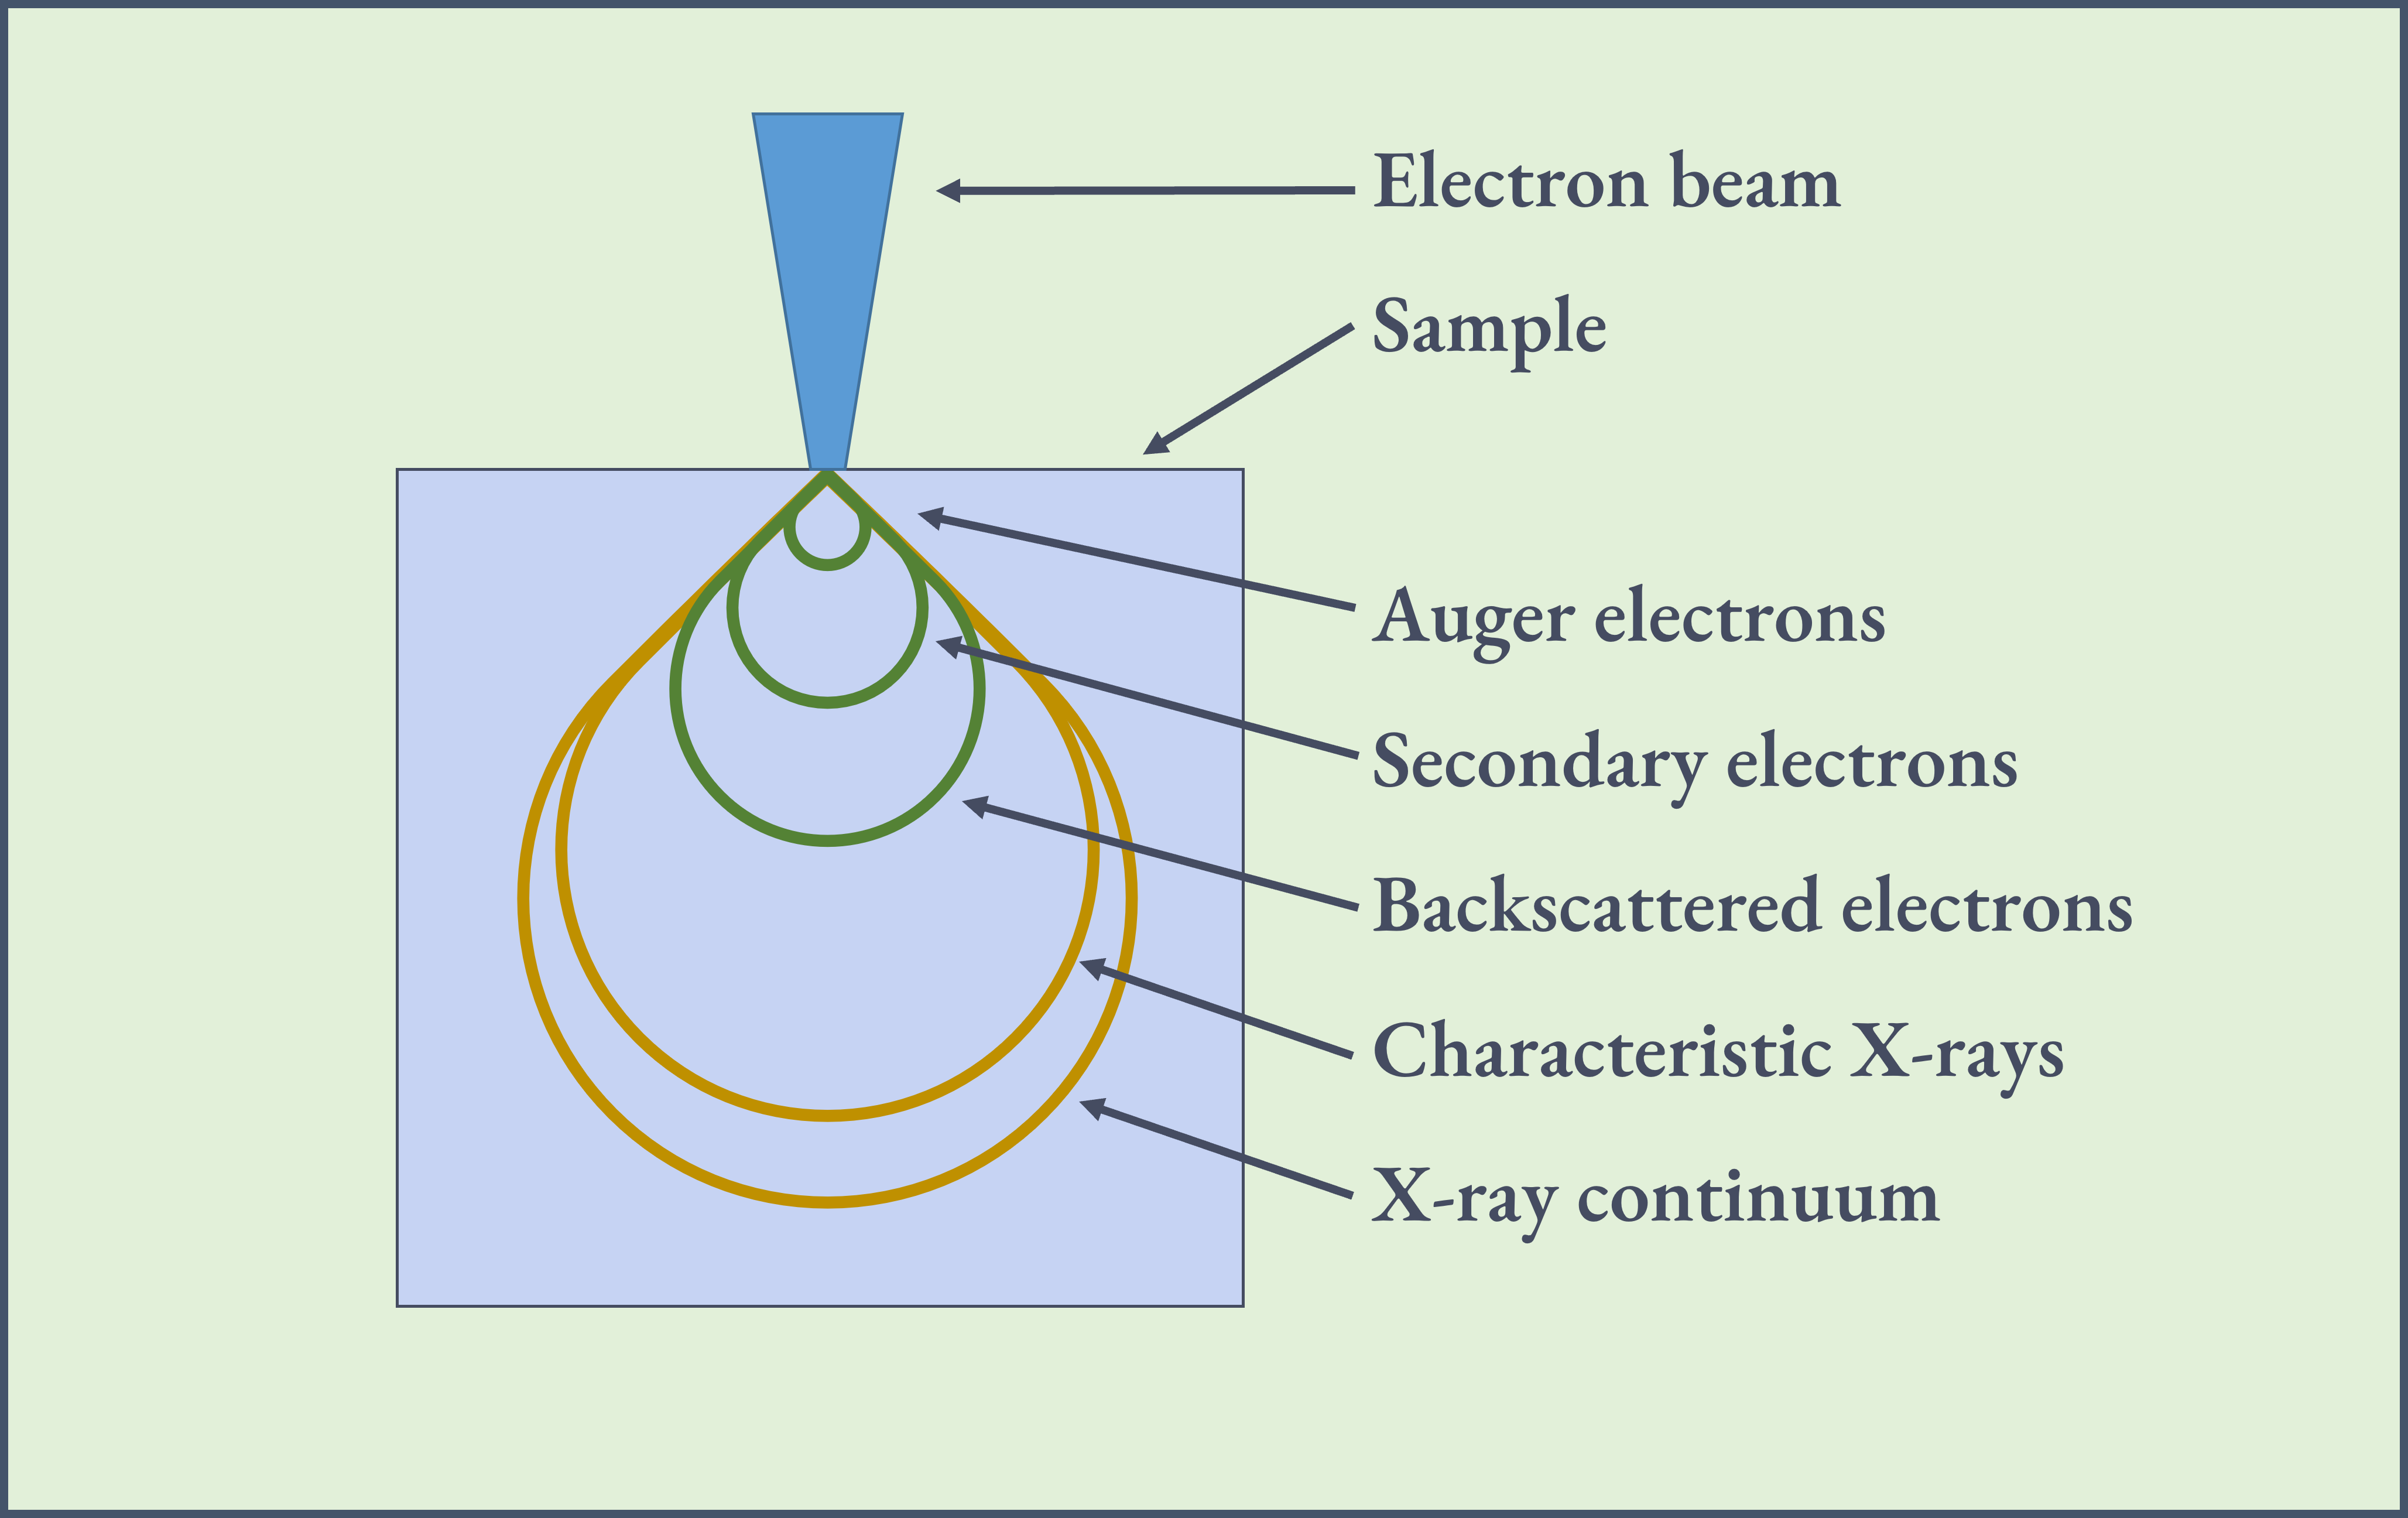
\includegraphics[width=0.8\linewidth]{figures/interaction_volume.png}
    \caption{
        Illustration of the interaction volume of the different signals.
        The signals are emitted in all directions, which is why the interaction volume is spherical.
        The blue signals are electrons and the orange signals are X-rays.
        The depths are not to scale.
    }
    \label{fig:interaction_volume}
\end{figure}


% \ton{Do you want me to write about the different signals, ie. SE and BSE?}


% The parts in the SEM
An SEM consists of several parts, which are illustrated in \cref{fig:SEM_setup}.
The electron gun is the source of the electrons.
The condenser lens focuses the electrons to a small beam.
The two apertures sets the size of the beam, which is important since the electrons closest to the central axis of the beam have fewest aberrations.
The scanning coils are used to scan the beam over the sample in the raster fashion.
The objective lens focuses the beam to a small spot on the sample.
In general a smaller spot allows higher resolution, because the signal is recorded from a smaller area.
However, this effect is limited by several factors, such as the interaction volume.
The detectors are placed above the sample.

% \ton{What more do you want me to write about the SEM?}

% figure/SEM_setup.png
\begin{figure}[ht]
    \centering
    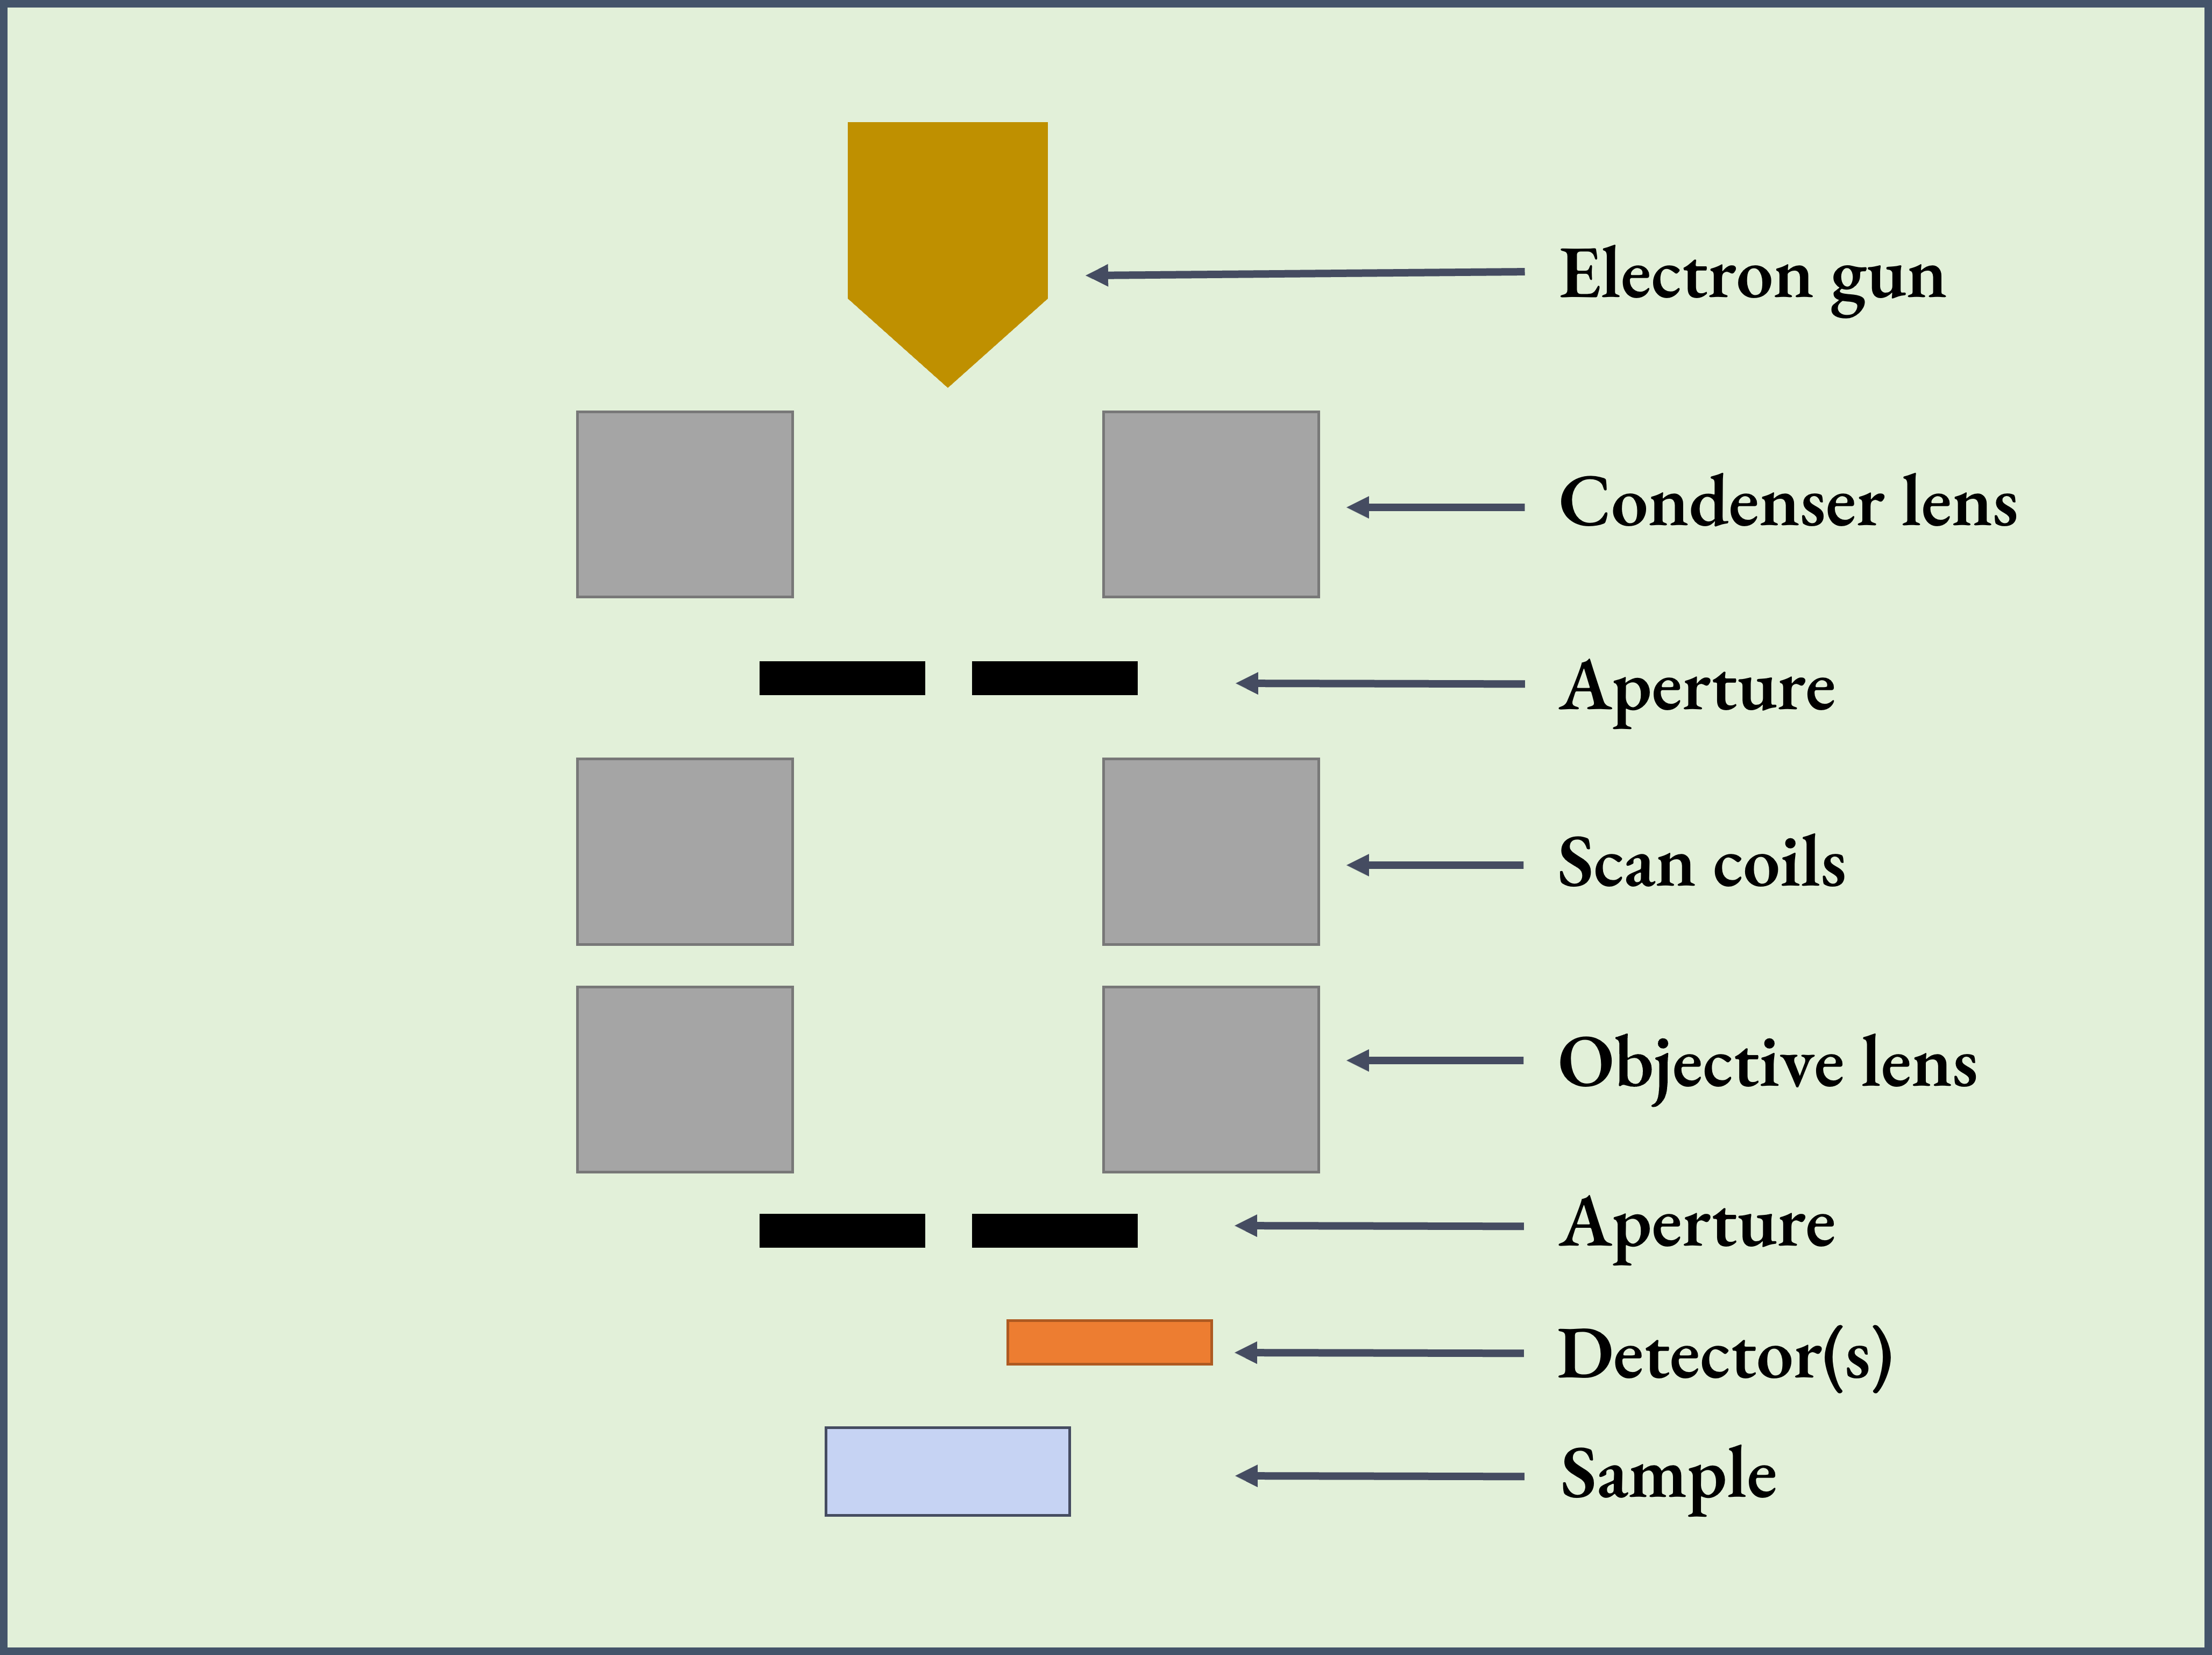
\includegraphics[width=0.8\linewidth]{figures/SEM_setup.png}
    \caption{
        Illustration of the parts in an SEM.
    }
    \label{fig:SEM_setup}
\end{figure}








\subsection{EDS}

% figure with x,y,z, azumuthal angle, WD, etc. See DTSA-II Figure 5
% file:///C:/Users/Brynjar/Documents/Masteroppgave/potensielle%20kilder/getting-started-with-nist-dtsa-ii%20(2).pdf 




% write about geometry in EDS, feedback


% write about escape depth of different materials.
% the absorption in the sample makes the escape depth of light elements shallow. Eg. Li have an escape depth of only a few nm (Keith Thompson, Is Energy Resolution Still an Important Specification in EDS?)


% explain counts input
% explain counts output




% section "instruments" end




\section{Quality control - detector characterization}
\label{theory:qc}

\brynjar{Do not use quality control, Ton does not like it. Health check?}

The aim of this work is to improve EDS bulk quantification, and one way to do this is to do a health check of the EDS set up.
A health check can both reveil errors in the setup and make the input parameters of the quantification more accurate.
Manufacturers of EDS detectors like Oxford Instruments provide a guide for how to perform quality control on their detector, but these guides focus on calibration of energy resolution and scale \cite{aztec_manual}.
The state of an EDS setup is characterized by more than its energy resolution and scale \cite{goldstein_scanning_2018}
Little literature is published on quality control programs for SEM EDS setups, but there are several papers on tests for TEM EDS.
% Mari: The tests are described by Watanabe in [30] and in the info-sheet by Ted Pella [33] which is based on the original work by R.F. Egerton and C.S. Cheng from 1994 [16].
% The complete test routine has several characteristics. Here only the most essential to this work are discussed, and an overview is found in Tab. 2.3.
One of the challenges in this work is to find the find the most relevant test characteristics, and what ranges of values are acceptable for a healthy detector.
Each test characteristics is described with what it is, how it is measured, and what values are acceptable.



\subsection{Duane-Hunt limit}
\label{theory:qc:duanehunt}
% put after calibration? It is done before in the code, but it is not a part of AZtec.

% What
The Duane-Hunt limit originates from a paper from Duane and Hunt in 1915 \cite{Duane_Hunt_1915}, and the Duane-Hunt limit is the maximum energy of the X-ray background radiation.
The Duane-Hunt limit is the indicent beam energy, E$_0$. \brynjar{Ref E$_1$ in figure/previous theory?}
The acceleration voltage from the instrument is the nominal beam energy, while the effective beam energy is the Duane-Hunt limit, and these two values can deviate significantly.
As seen in \cref{fig:duanehunt}, the detected X-rays decline rapidly and linearly towards the beam energy, but the counts does not go to zero.
It is not possible to excite X-rays above the beam energy, thus the spectrum should be cut off at the beam energy to allow better model fitting.
The counts above the Duane-Hunt limit are due to coincidence counts, where two X-rays are detected as one.
The tail of coincidence counts makes the exact beam energy is ambiguous, which is solved by calculating the Duane-Hunt limit as a linear fit of the background, and the beam energy is the intersection of the linear fit and the x-axis \cite{software_dtsaii} \cite[Ch. 9.1.3]{goldstein_scanning_2018}.

% figures/Duane-Hunt.png
\begin{figure}[ht]
    \centering
    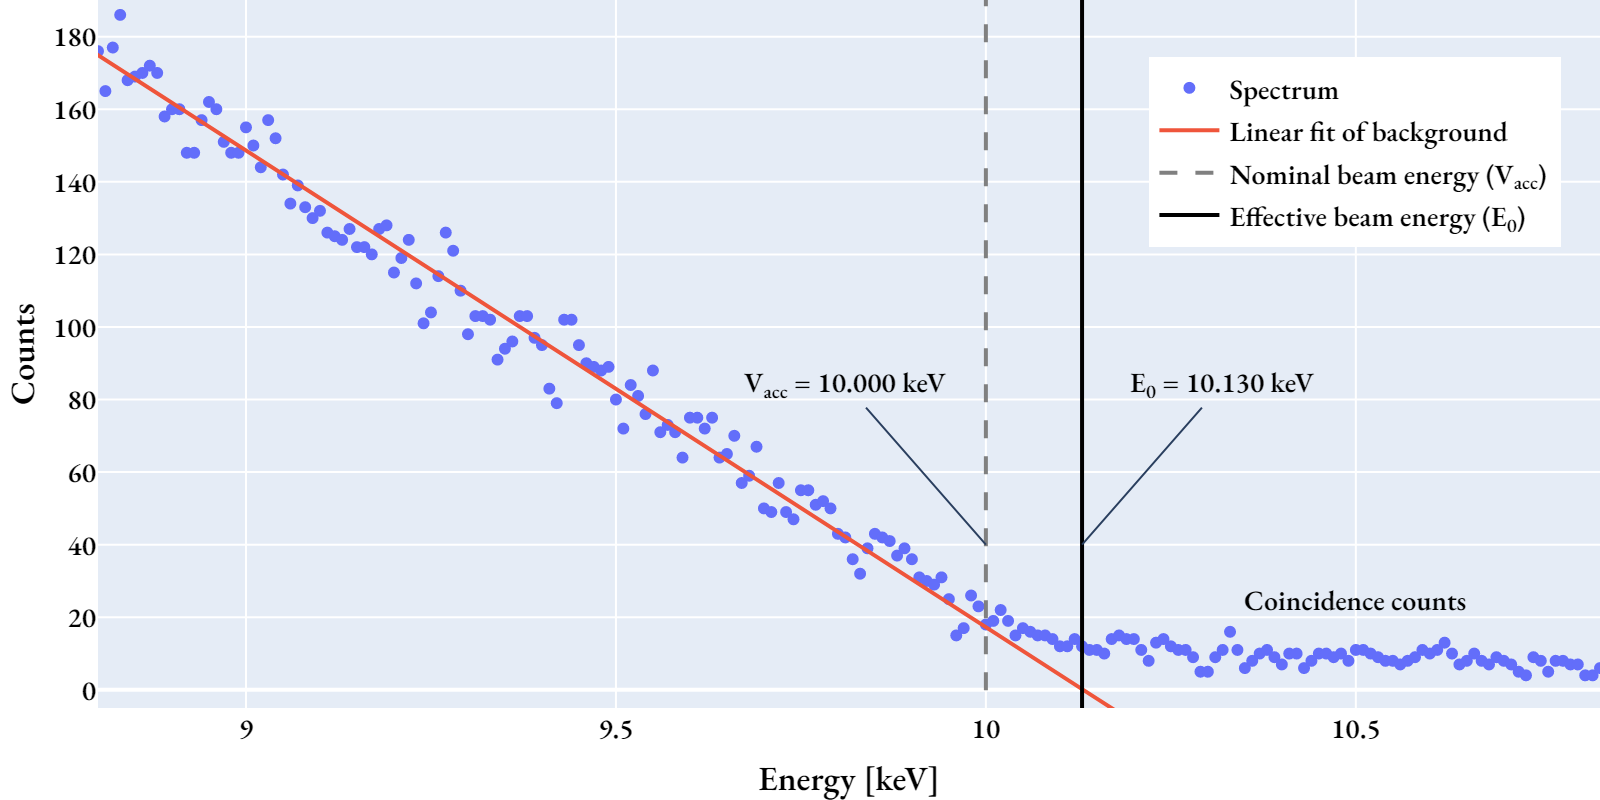
\includegraphics[width=0.8\linewidth]{figures/Duane-Hunt.png}
    \caption{
        Illustration of the Duane-Hunt limit.
        The blue dots are the X-ray counts, and the red line is a linear fit of the background.
        The gray dashed line is the nominal beam energy, and the black line is the effective beam energy.
    }
    \label{fig:duanehunt}
\end{figure}

% How
% covered above

% Acceptable values
There will be some deviation between the nominal beam energy and the effective beam energy, typically up to 0.2 keV.
Different specimen will have different deviation, due to varying conductivity.
Specimen with low conductivity will get problems with charging, which will lowers the effective beam energy.
Thus, a deviation between the nominal and effective beam energy of several kilo-electronvolts is a sign of charging \cite{dtsaii_2_manipulating_spectra}.
Charging of specimen are covered in detail in a paper by Postek and Vladár \cite{postek_charging_2015}.






\subsection{Calibration of energy resolution}
\label{theory:qc:energyres}

\brynjar{Remove "Calibration of"? Also for the next two}

% What
The energy resolution of an EDS system is the ability to distinguish two lines at different energies, and is measured by the FWHM of the Mn K$\alpha$ peak.
The convention of using the Mn K$\alpha$ peak as the reference for the energy resolution is its position at 5.8987 keV, which gives an indication for both the lower and higher energies used in EDS.
The first SDD \brynjar{(explain earlier in EDS part)} detectors had an energy resolution between 160 and 200 eV, while modern detectors can achieve energy resolution lower than 120 eV, which allow closer peaks to be seperated \cite{keith_energy_res_2013} \brynjar{(Thompson refers to Goldstein\dots)}.
An instrument is stated to have a certain energy resolution, however the actual resolution of a given spectrum varies with the acquisition settings.
In \cite{keith_energy_res_2013} Thompson show that with constand dead time a higher input count rate gives worse resolution, with the example of 121 eV resolution with <5000 cps, and 140-150 eV resolution with >100,000 cps.
Because of this, Thompson explains that EDS specifications are based on acquisition designs with low input counts.
Changes in dead time are also affecting the energy resolution, where shorter dead time give degraded resolution, because a lower dead time gives the computer shorter time to process the incoming signal and sets the channel value less accurate of each count \brynjar{Ref?}.


% What is the energy resolution.
% What is a good energy resolution.
% Why Mn K$\alpha$?
% Finding the calibrated energy resolution, Mn K$\alpha$.

% Approaching the theoretical limit? Find source, Goldstein?
% TODO: amplifier noise is described with an equation in Woldseth 1973, referenced in bennett_egerton_1995.
% Woldseth 1973 figure remake in Goldstein 2003 3rd ed.: It can readily be seen that even if the noise contribution were totally eliminated, the theoretical energy resolution limit would still be greater than 100 eV for Fe Ka at 6.4 keV

% How

% Direct measurement
\brynjar{Implement check for Mn K$\alpha$ peak in the code.}
The most straight forward way of finding a detectors energy resolution is to measure the FWHM of the Mn K$\alpha$ peak in a sample with Mn, preferably with high concentration as that provides more defined peaks.
The FWHM measurement should be from a Gaussian fit of the peak, because of variations in the count statistics as explained in \verb|\cref{gaussian_something}| \brynjar{fix internal reference}.
\brynjar{One paragraph for each method?}


% Ni Ka * 0.926
Another approach, which can be used when a sample with Ni is avaliable, is to measure the FWHM of Ni K$\alpha$ and multiply the value with 0.926 \cite{bennett_egerton_1995}.
This approach is based on a study in 1995 where five TEM laboratories were given a NiO test specimen with a series of EDS test measurements to be done, where one of the tests were focused on the energy resolution.
The test used the Ni K$\alpha$ and O K$\alpha$ peaks, where the FWHM of these two lines were measured, and a linear correlation between photon energy and the square of the energy resoltion was assumed.
Then the FWHM of Mn K$\alpha$ was determined by interpolation, and the factor 0.926 was reported as a sufficiently good conversion between Ni K$\alpha$ and Mn K$\alpha$.


% HyperSpy
A third and more general approach, is to use the energy calibration method in HyperSpy, which estimates the FWHM of Mn K$\alpha$.
The method, \verb|m.calibrate_energy_axis(calibrate='resolution', xray_lines='all_alpha')|, is used on a model of a spectrum and does the estimation in two steps.
The first step is to fit the width of all the lines in the spectrum, which is needed to get a correct reference peak width, i.e. an account for the peak broadening of the detector \ton{This I read from the HS code, line 50 in: \url{https://github.com/hyperspy/hyperspy/blob/842d6d9713d866960a033d4006200a43841079fe/hyperspy/models/edsmodel.py}}.
The second step utilize an equation from Fiori and Newbury from 1978 (\brynjar{Fiori, C. E., and Newbury, D. E. (1978). In SEM/1978/I, SEM, Inc., AFM O'Hare, Illinois, p. 401.}), which calculates the FWHM of an given energy located anywhere in the spectrum by:

\begin{equation}
    \label{eq:estimateFWHM}
    \textnormal{FWHM} =  \sqrt{2.5 * (E - E_\textnormal{ref}) + \textnormal{FWHM}^2_{\textnormal{ref}}}
\end{equation}

Where $E$ is the energy of the wanted FWHM, i.e. Mn K$\alpha$.
$E_\textnormal{ref}$ is the energy of a reference line in the spectrum, and $\textnormal{FWHM}_{\textnormal{ref}}$ is the FWHM of that line.
When using the HyperSpy method \verb|calibrate_energy_axis|, the user should be aware of the argument \verb|xray_lines|, which can either be a list of strings with line names or \verb|'all_alpha'|, which is the default value for the argument.
As of HyperSpy v1.7.3, the reference line in \cref{eq:estimateFWHM} is the first line in \verb|xray_lines|, which is the alphabetically first alpha line when \verb|xray_lines='all_alpha'|.
The reference line must be a well defined peak for the method to work properly.
\brynjar{Discuss: when taking a series of spectra with different Vacc, the first line (eg AsKa in GaAs or AlKa in SU9000) is poorly defined for 10 kV and 5 kV respectively, resulting in weirdly poor Mn Ka estimate.}
\ton{I have examples where this does not work as intended, and I can suggest a change in HyperSpy to eg. use the line with highest counts as the reference. It took me some time to figure this out, but now I know what causes this.}


% links for HyperSpy:
% https://github.com/hyperspy/hyperspy/blob/842d6d9713d866960a033d4006200a43841079fe/hyperspy/models/edsmodel.py
% search for:
% % calibrate_energy_axis
% % _set_energy_resolution
% % _get_sigma


% Acceptable values
% TODO: run this by ton
\ton{This paragraph about acceptable values are bad. Any suggestions here?}
The energy resolution of a taken spectrum should be close to what the specifications of the EDS.
Deviations implicate \dots (High cps? Low DT? What else?)
As explained, the theoretical limit of the FWHM of Mn K$\alpha$ is XXX \brynjar{explain above!}.
The HyperSpy method will raise an ValueError if the estimated energy resolution is below 110 eV \brynjar{line 450, \url{https://github.com/hyperspy/hyperspy/blob/842d6d9713d866960a033d4006200a43841079fe/hyperspy/models/edsmodel.py}}.




\subsection{Calibration of scale and offset}
\label{theory:qc:scaleoffset}
% scale and offset in one subsection?

% What
What is the scale and offset.
Typical values for the scale.

% How
Measure two far apart peaks and find their distance in the spectrum.
Or, use the HS function, which does \dots

% Acceptable values
Deviations should be \dots
Large deviations implicate \dots


\subsection{Calibrating peak positions}
\label{theory:qc:peakpositions}

% What
What is the peak position.
Also mention the peak width?
Why does it deviate from the theoretical value.
Figure of Mo K$\alpha$ peak which is not centered?
Why bigger changes at higher energies.

% How
Manual: add gaussians at the expected position and fit.
HS: adds gaussians at the expected position and fit with the centre as free parameter.

% Acceptable values
Deviations can be higher at higher energies, but should be \dots
Large deviations implicate \dots


% one section on the calculated value for each line of interest?
% Line           True E [keV]   Calib. E [keV] Area [counts]  Max (fit)      Sigma [keV]    FWHM [eV]      Fiori P_10/B

\subsection{Fiori peak to background ratio}
\label{theory:qc:fiori}


\subsection{Peak ratio}
\label{theory:qc:peakratio}
% contaminations, at least for TEM: change of Ka/La, eg in Ni
% also used for stray radiation measurements 
% stray intensity: (Ni Ka/Mo Ka) 
% stray predominent source: (Mo Ka/Mo La), only for TEM?

% the flexibility, since eg a pure Cu sample will give some statistics but not stray information.


\subsection{Peak shape}
\label{theory:qc:peakshape}
% The real lines are Lorentzians with width of 1-10 eV, but the peaks are wider due to electronic noise.
% Peaks are gaussians by electronic noise.
% a measure of the peak shape is the FWTM/FWHM


\subsection{Number of counts in peaks vs background}
\label{theory:qc:counts}

% Total counts, background counts.
% How to represent the measure better? Ratio, percentage, absolute value, etc.
% Fiori P/B is a measure already covered.


\subsection{Stray radiation measurements - when possible}
\label{theory:qc:stray}
% both intensity and source.
% intensity:  a major line and a stray line.
% source:  Mo Ka and Mo La ratio



% The two most important tests, according to Goldstein, are linearity and stability.
% requires multiple spectra of the same sample with different beam currents.
% Goldstein p. 232.








%%%%%%%%%%%%%%%%%





%%%%%%%% EDS Issues
% Several issues can perturb an EDS spectrum, including peak broadening, peak distortion, silicon x-ray escape peaks, absorption edges, and the silicon internal fluorescence peak. In addition, several hardware-related problems, such as pulse pileup rejection by the main amplifier, acoustic coupling on the co-axial connector between the detector and the amplifier, ground loops, and ice in the detector system, can occur.
% https://www.semitracks.com/reference-material/failure-and-yield-analysis/failure-analysis-materials-characterization/energy-dispersive-x-ray-spectrometry.php#:~:text=History,used%20for%20x%2Dray%20characterization.
